\documentclass{article}

\usepackage{polski}
\usepackage[utf8]{inputenc}

\usepackage{fancyhdr} % Required for custom headers
\usepackage{lastpage} % Required to determine the last page for the footer
\usepackage{extramarks} % Required for headers and footers
\usepackage[usenames,dvipsnames]{color} % Required for custom colors
\usepackage{graphicx} % Required to insert images
\usepackage{listings} % Required for insertion of code
\usepackage{courier} % Required for the courier font
\usepackage{lipsum} % Used for inserting dummy 'Lorem ipsum' text into the template\
\usepackage{amsfonts}
\usepackage{amsthm}
\usepackage{hyperref}
\usepackage{tikz}
\usepackage{amsmath}
\usepackage{pdfpages}
\usepackage{mathtools}


\newtheorem{thm}{Twierdzenie}
\newtheorem{remark}{Uwaga}
\newtheorem{lemat}{Lemat}


\newenvironment{prooff}{\paragraph{Dowód:}}{\hfill$\square$}
\newenvironment{rozw}{\paragraph{Rozwiazanie:}}{\hfill}

% Margins
\topmargin=-0.45in
\evensidemargin=0in
\oddsidemargin=0in
\textwidth=6.5in
\textheight=9.0in
\headsep=0.25in

\linespread{1.1} % Line spacing

% Set up the header and footer
\pagestyle{fancy}
\lhead{\hmwkAuthorName} % Top left header
\chead{\hmwkClass\ (\hmwkClassInstructor\ \hmwkClassTime): \hmwkTitle} % Top center head
\rhead{\firstxmark} % Top right header
\lfoot{\lastxmark} % Bottom left footer
\cfoot{} % Bottom center footer
\rfoot{Page\ \thepage\ of\ \protect\pageref{LastPage}} % Bottom right footer
\renewcommand\headrulewidth{0.4pt} % Size of the header rule
\renewcommand\footrulewidth{0.4pt} % Size of the footer rule

\setlength\parindent{0pt} % Removes all indentation from paragraphs
%----------------------------------------------------------------------------------------
%	DOCUMENT STRUCTURE COMMANDS
%	Skip this unless you know what you're doing
%----------------------------------------------------------------------------------------

% Header and footer for when a page split occurs within a problem environment
\newcommand{\enterProblemHeader}[1]{
\nobreak\extramarks{#1}{#1 continued on next page\ldots}\nobreak
\nobreak\extramarks{#1 (continued)}{#1 continued on next page\ldots}\nobreak
}

% Header and footer for when a page split occurs between problem environments
\newcommand{\exitProblemHeader}[1]{
\nobreak\extramarks{#1 (continued)}{#1 continued on next page\ldots}\nobreak
\nobreak\extramarks{#1}{}\nobreak
}

\setcounter{secnumdepth}{0} % Removes default section numbers
\newcounter{homeworkProblemCounter} % Creates a counter to keep track of the number of problems

\newcommand{\homeworkProblemName}{}
\newenvironment{homeworkProblem}[1][Zadanie \arabic{homeworkProblemCounter}]{ % Makes a new environment called homeworkProblem which takes 1 argument (custom name) but the default is "Problem #"
\stepcounter{homeworkProblemCounter} % Increase counter for number of problems
\renewcommand{\homeworkProblemName}{#1} % Assign \homeworkProblemName the name of the problem
\section{\homeworkProblemName} % Make a section in the document with the custom problem count
\enterProblemHeader{\homeworkProblemName} % Header and footer within the environment
}{
\exitProblemHeader{\homeworkProblemName} % Header and footer after the environment
}

\newcommand{\problemAnswer}[1]{ % Defines the problem answer command with the content as the only argument
\noindent\framebox[\columnwidth][c]{\begin{minipage}{0.98\columnwidth}#1\end{minipage}} % Makes the box around the problem answer and puts the content inside
}

\newcommand{\homeworkSectionName}{}
\newenvironment{homeworkSection}[1]{ % New environment for sections within homework problems, takes 1 argument - the name of the section
\renewcommand{\homeworkSectionName}{#1} % Assign \homeworkSectionName to the name of the section from the environment argument
\subsection{\homeworkSectionName} % Make a subsection with the custom name of the subsection
\enterProblemHeader{\homeworkProblemName\ [\homeworkSectionName]} % Header and footer within the environment
}{
\enterProblemHeader{\homeworkProblemName} % Header and footer after the environment
}

\usepackage{listings} % Required for inserting code snippets
\usepackage[usenames,dvipsnames]{color} % Required for specifying custom colors and referring to colors by name

\definecolor{DarkGreen}{rgb}{0.0,0.4,0.0} % Comment color
\definecolor{highlight}{RGB}{255,251,204} % Code highlight color

\lstdefinestyle{Style1}{ % Define a style for your code snippet, multiple definitions can be made if, for example, you wish to insert multiple code snippets using different programming languages into one document
language=Perl, % Detects keywords, comments, strings, functions, etc for the language specified
backgroundcolor=\color{highlight}, % Set the background color for the snippet - useful for highlighting
basicstyle=\footnotesize\ttfamily, % The default font size and style of the code
breakatwhitespace=false, % If true, only allows line breaks at white space
breaklines=true, % Automatic line breaking (prevents code from protruding outside the box)
captionpos=b, % Sets the caption position: b for bottom; t for top
commentstyle=\usefont{T1}{pcr}{m}{sl}\color{DarkGreen}, % Style of comments within the code - dark green courier font
deletekeywords={}, % If you want to delete any keywords from the current language separate them by commas
%escapeinside={\%}, % This allows you to escape to LaTeX using the character in the bracket
firstnumber=1, % Line numbers begin at line 1
frame=single, % Frame around the code box, value can be: none, leftline, topline, bottomline, lines, single, shadowbox
frameround=tttt, % Rounds the corners of the frame for the top left, top right, bottom left and bottom right positions
keywordstyle=\color{Blue}\bf, % Functions are bold and blue
morekeywords={}, % Add any functions no included by default here separated by commas
numbers=left, % Location of line numbers, can take the values of: none, left, right
numbersep=10pt, % Distance of line numbers from the code box
numberstyle=\tiny\color{Gray}, % Style used for line numbers
rulecolor=\color{black}, % Frame border color
showstringspaces=false, % Don't put marks in string spaces
showtabs=false, % Display tabs in the code as lines
stepnumber=5, % The step distance between line numbers, i.e. how often will lines be numbered
stringstyle=\color{Purple}, % Strings are purple
tabsize=2, % Number of spaces per tab in the code
}

% Create a command to cleanly insert a snippet with the style above anywhere in the document
\newcommand{\insertcode}[2]{\begin{itemize}\item[]\lstinputlisting[caption=#2,label=#1,style=Style1]{#1}\end{itemize}} % The first argument is the script location/filename and the second is a caption for the listing

%----------------------------------------------------------------------------------------
%	NAME AND CLASS SECTION
%----------------------------------------------------------------------------------------

\newcommand{\hmwkTitle}{Lista 2} % Assignment title
\newcommand{\hmwkDueDate}{} % Due date
\newcommand{\hmwkClass}{Matematyka dyskretna} % Course/class
\newcommand{\hmwkClassTime}{Czw 16-19} % Class/lecture time
\newcommand{\hmwkClassInstructor}{Krzysztof Nowicki} % Teacher/lecturer
\newcommand{\hmwkAuthorName}{Bartosz Bednarczyk} % Your name

%----------------------------------------------------------------------------------------
%	TITLE PAGE
%----------------------------------------------------------------------------------------

\title{
\vspace{2in}
\textmd{\textbf{\hmwkClass:\ \hmwkTitle}}\\
\normalsize\vspace{0.1in}\small{Due\ on\ \hmwkDueDate}\\
\vspace{0.1in}\large{\textit{\hmwkClassInstructor\ \hmwkClassTime}}
\vspace{3in}
}

\author{\textbf{\hmwkAuthorName}}
\date{} % Insert date here if you want it to appear below your name

%----------------------------------------------------------------------------------------

\begin{document}


%----------------------------------------------------------------------------------------
%	TABLE OF CONTENTS
%----------------------------------------------------------------------------------------

\begin{center}
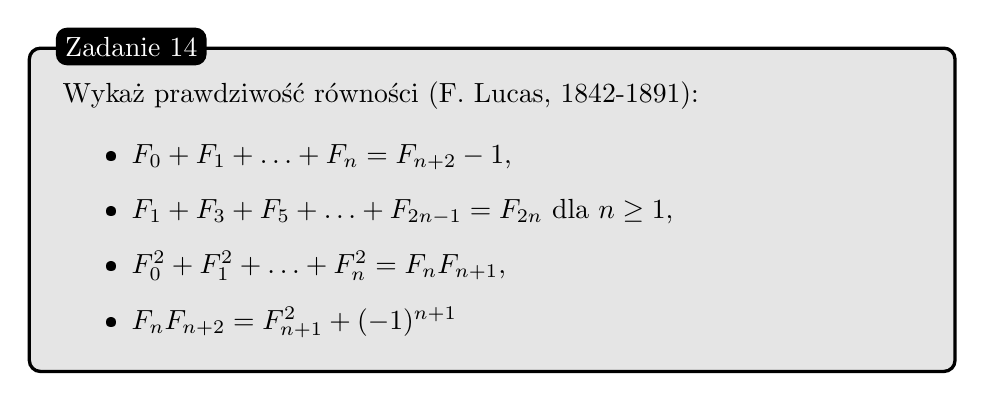
\begin{tikzpicture}
\node [draw={black}, fill=black!10, very thick, rectangle, rounded corners, inner sep=12pt, inner ysep=12pt] (box){%
    \begin{minipage}{.9\textwidth}
    Wykaż prawdziwość równości (F. Lucas, 1842-1891):

    \begin{itemize}
    \item $F_0 + F_1 + \ldots + F_n = F_{n+2} - 1$,
    \item $F_1 + F_3 + F_5 + \ldots + F_{2n-1} = F_{2n}$ dla $n \geq 1$,
    \item $F_0^2 + F_1^2 + \ldots + F_n^2 = F_nF_{n+1}$,
    \item $F_nF_{n+2} = F_{n+1}^2 + (-1)^{n+1}$
    \end{itemize}

    \end{minipage}
};
\node[fill={black}, text=white, rounded corners, right=10pt] at (box.north west) {Zadanie 14};
\end{tikzpicture}
\end{center}

\begin{thm}
$F_0 + F_1 + \ldots + F_n = F_{n+2} - 1$
\end{thm}
\begin{proof}
Przeprowadźmy dowód indukcyjny względem $n$. Niech $X = \lbrace n \in \mathbb{N} \ | \ \sum_{i=0}^n F_i = F_{n+2} - 1 \rbrace$. Zauważmy, że $0 \in X$, ponieważ $\sum_{i=0}^n F_i = F_0 = 0 = 1 -1 = F_2 - 1 = F_{0+2} - 1$.
Weźmy dowolne $n \in \mathbb{N}$. Załóżmy, że $n \in \mathbb{N}$ i pokażmy, że $n+1 \in X$.

$$\sum_{i=0}^{n+1} F_i = F_{n+1} + \sum_{i=0}^n F_i \stackrel{zal}{=} F_{n+1} + F_{n+2} - 1 = F_{(n+1) + 2} - 1$$

Z powyższych rachunków wynika, że $n+1 \in X$. Zatem na mocy zasady indukcji matematycznej $X = \mathbb{N}$, czyli twiedzenie 1 jest prawdziwe dla dowolnego naturalnego $n$.
\end{proof}

\begin{thm}
$F_1 + F_3 + F_5 + \ldots + F_{2n-1} = F_{2n}$ dla $n \geq 1$
\end{thm}
\begin{proof}
Weźmy dowolne $n \in \mathbb{N}_+$. Wiemy, że $F_i + F_{i+1} = F_{i+2}$. Zatem:

$$
F_1 + F_3 + F_5 + \ldots + F_{2n-1} = F_{2n} = \underline{0 + F_1} + F_3 + F_5 + \ldots + F_{2n-1} = F_{2n} = \underline{F_2 + F_3} + F_5 + \ldots + F_{2n-1} = 
$$
$$
= \underline{F_4 + F_5} + F_7 + \ldots + F_{2n-1} = \underline{F_6 + F_7} + F_9 + \ldots + F_{2n-1} = \ldots = \underline{F_{2n-2} + F_{2n-1}} = F_{2n}
$$
\end{proof}

\begin{thm}
$F_0^2 + F_1^2 + \ldots + F_n^2 = F_nF_{n+1}$
\end{thm}
\begin{proof}
Indukcyjnie względem $n$. Zdefiniujmy $X$ jako $\lbrace n \in \mathbb{N} \ | \ \sum_{i=0}^n F_i^2 = F_nF_{n+1} \rbrace$.\\
$0 \in X$, ponieważ $\sum_{i=0}^n F_i^2 = F_0^2 = 0 = 0 \cdot 1 = F_0 F_{0+1}$.
Weźmy dowolne $n \in \mathbb{N}$. Załóżmy, że $n \in X$. Pokażmy, że $n+1 \in X$.

$$\sum_{i=0}^{n+1} F_i^2 = F_{n+1}^2 + \sum_{i=0}^n F_i^2 \stackrel{zal}{=} F_{n+1}^2 + F_nF_{n+1} = F_{n+1} \cdot \left( F_{n+1} + F_n \right) = F_{n+1}F_{n+2}$$

$n+1 \in X$. Zatem z zasady indukcji wiemy, że $X = \mathbb{N}$, co pociąga za sobą prawdziwość twierdzenia nr 3.

\end{proof}

\begin{thm}
$F_nF_{n+2} = F_{n+1}^2 + (-1)^{n+1}$
\end{thm}
\begin{proof}

Przeprowadźmy dowód indukcyjnie. $n$. Niech $X = \lbrace n \in \mathbb{N} \ | \ F_nF_{n+2} = F_{n+1}^2 + (-1)^{n+1} \rbrace$. Zauważmy że  $0 \in X$, ponieważ $F_0F_{n+2} = 0 = 1^2 - 1 =  F_{0+1}^2 + (-1)^{0+1}$.


Weźmy dowolne $n \in \mathbb{N}$. Załóżmy, że $n \in X$. Pokażmy, że $n+1 \in X$.

$$F_{n+2}F_n - F_{n+1}^2 = \left( F_{n+1} + F_n \right) F_n - F_{n+1}^2 = F_n^2 + F_{n+1} F_n - F_{n+1}^2 = $$

$$= F_n^2 - F_{n+1} \left( F_{n+1} - F_n \right) = F_n^2 - F_{n+1} F_{n-1} = -1 \cdot (-1)^n = \left( -1 \right)^{n+1}$$ 

Z powyższych rachunków $n+1 \in X$, zatem podany wzór jest prawdziwy dla dowolnego $n \in \mathbb{N}$.

\end{proof}


%----------------------------------------------------------------------------------------

\end{document}